\documentclass[tikz,border=10pt]{standalone}
\usetikzlibrary{arrows.meta, positioning, shapes.geometric, shapes.misc, fit, backgrounds, calc, matrix}

\tikzset{
    >=Latex,
    font=\sffamily\large,
    node distance=1.5cm and 3cm,
    dag_result/.style={
        rectangle, 
        draw=green!70!black, 
        fill=green!15, 
        very thick, 
        minimum width=4.5cm, 
        minimum height=1.5cm, 
        text width=5cm,
        align=center
    },
    dag_lemma/.style={
        rounded rectangle, 
        draw=orange!80!black, 
        fill=yellow!20, 
        very thick, 
        minimum width=4.5cm, 
        minimum height=1.5cm, 
        text width=5cm,
        align=center
    },
    dag_model/.style={
        ellipse, 
        draw=blue!70!black, 
        fill=blue!12, 
        very thick, 
        minimum width=4.5cm, 
        minimum height=1.5cm, 
        text width=4.5cm,
        align=center
    },
    dag_unformalized/.style={
        rectangle, 
        draw=gray!60!black, 
        fill=gray!10, 
        very thick, 
        dashed, 
        minimum width=4.5cm, 
        minimum height=1.5cm, 
        text width=5cm,
        align=center
    },
    dag_conditional/.style={
        rectangle, 
        rounded corners,
        draw=orange!80!black, 
        fill=orange!10, 
        very thick, 
        minimum width=4.5cm, 
        minimum height=1.5cm, 
        text width=5cm,
        align=center
    },
    dag_partial/.style={
        rectangle,
        rounded corners,
        draw=yellow!55!black,
        fill=yellow!10,
        very thick,
        dashed,
        minimum width=4.5cm,
        minimum height=1.5cm,
        text width=5cm,
        align=center
    },
    dag_scaffold/.style={
        rectangle,
        draw=gray!55!black,
        fill=white,
        very thick,
        dotted,
        minimum width=4.5cm,
        minimum height=1.5cm,
        text width=5cm,
        align=center
    },
    dag_caveat/.style={
        diamond, 
        draw=red!70!black, 
        fill=red!10, 
        minimum width=4cm, 
        align=center, 
        inner sep=0pt, 
        font=\sffamily\small
    },
    dag_arrow/.style={
        -{Stealth[scale=1.2]}, 
        very thick,
        shorten >=1.5pt,
        shorten <=1.5pt
    },
    dag_dashed_arrow/.style={
        -{Stealth[scale=1.2]}, 
        very thick, 
        dashed,
        shorten >=1.5pt,
        shorten <=1.5pt
    },
    dag_template_legend/.style={
        minimum width=2.6cm,
        minimum height=0.8cm,
        text width=2.45cm,
        inner sep=3pt,
        font=\sffamily\small,
        align=center
    },
    dag_template_note/.style={
        rectangle,
        draw=gray!50,
        fill=gray!5,
        rounded corners,
        text width=13cm,
        align=left,
        font=\sffamily\small,
        inner sep=6pt
    }
}

% Legend Helper
\newcommand{\daglegend}[2]{
    \node[draw, rounded corners, very thick, fit=#1, inner sep=12pt, label=above:\textbf{\Large Legend}] (#2) {};
}


\begin{document}
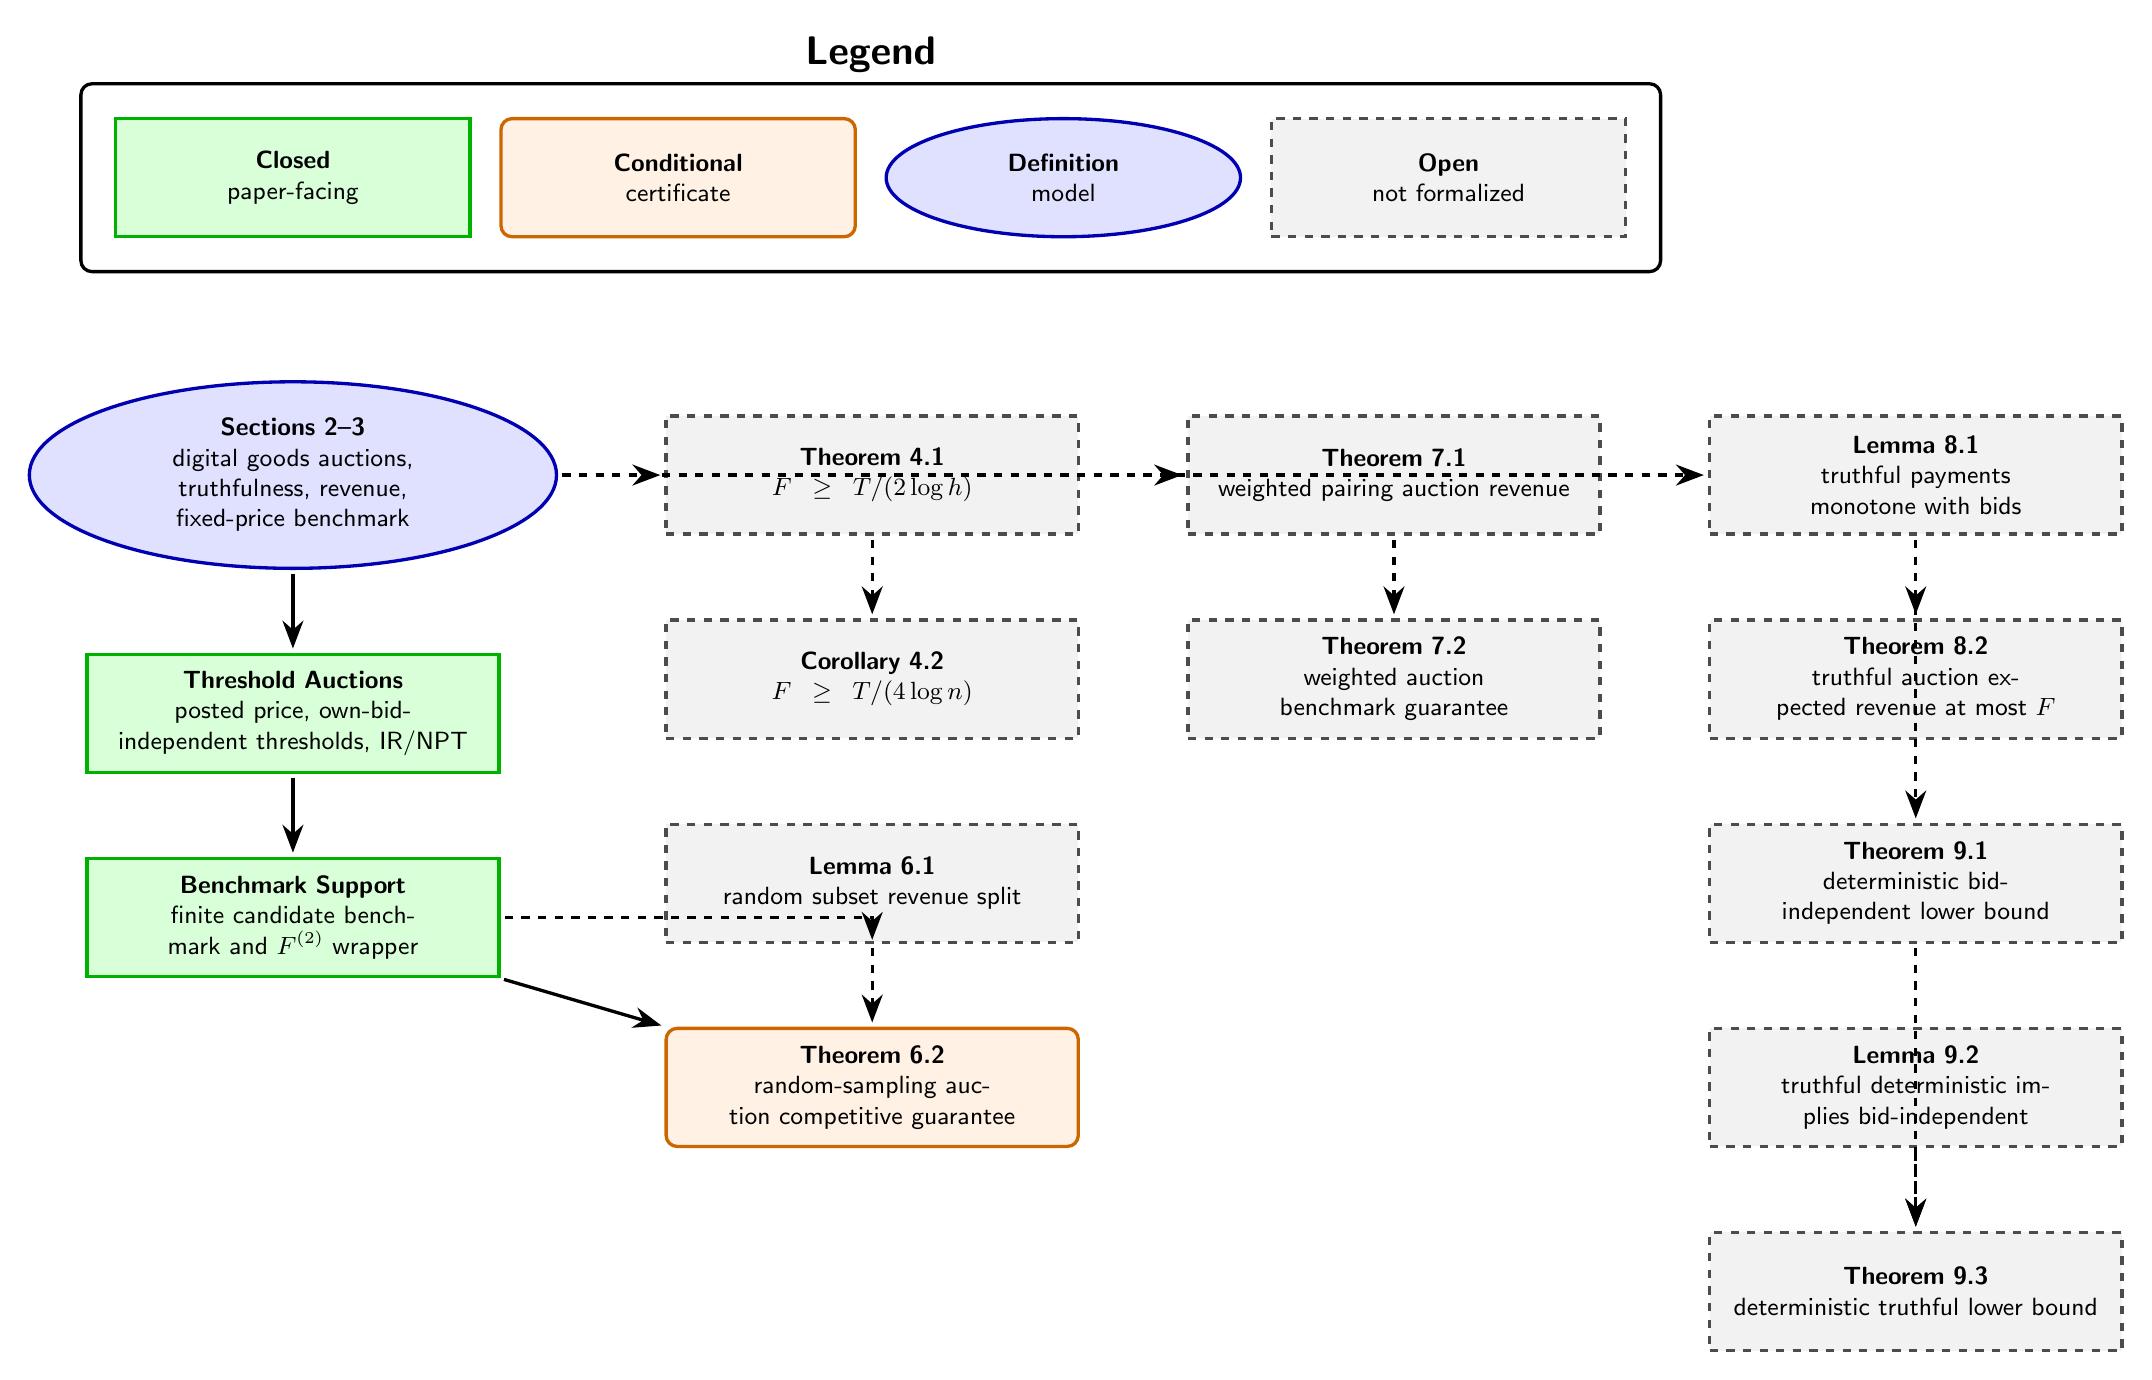
\begin{tikzpicture}[node distance=1.05cm and 1.35cm,
  every node/.style={font=\sffamily\small}]

\node[dag_result, text width=2.9cm] (legRes) {\textbf{Closed}\\paper-facing};
\node[dag_conditional, right=0.35cm of legRes, text width=2.9cm] (legCond) {\textbf{Conditional}\\certificate};
\node[dag_model, right=0.35cm of legCond, text width=2.9cm] (legDef) {\textbf{Definition}\\model};
\node[dag_unformalized, right=0.35cm of legDef, text width=2.9cm] (legOpen) {\textbf{Open}\\not formalized};
\daglegend{(legRes)(legCond)(legDef)(legOpen)}{Legend}

\node[dag_model, below=1.8cm of legRes] (Defs)
  {\textbf{Sections 2--3}\\digital goods auctions, truthfulness, revenue, fixed-price benchmark};
\node[dag_result, below=of Defs] (Threshold)
  {\textbf{Threshold Auctions}\\posted price, own-bid-independent thresholds, IR/NPT};
\node[dag_result, below=of Threshold] (Benchmark)
  {\textbf{Benchmark Support}\\finite candidate benchmark and $F^{(2)}$ wrapper};

\node[dag_unformalized, right=of Defs] (Thm41)
  {\textbf{Theorem 4.1}\\$F \ge T/(2\log h)$};
\node[dag_unformalized, below=of Thm41] (Cor42)
  {\textbf{Corollary 4.2}\\$F \ge T/(4\log n)$};
\node[dag_unformalized, below=of Cor42] (Lemma61)
  {\textbf{Lemma 6.1}\\random subset revenue split};
\node[dag_conditional, below=of Lemma61] (Thm62)
  {\textbf{Theorem 6.2}\\random-sampling auction competitive guarantee};

\node[dag_unformalized, right=of Thm41] (Thm71)
  {\textbf{Theorem 7.1}\\weighted pairing auction revenue};
\node[dag_unformalized, below=of Thm71] (Thm72)
  {\textbf{Theorem 7.2}\\weighted auction benchmark guarantee};

\node[dag_unformalized, right=of Thm71] (Lemma81)
  {\textbf{Lemma 8.1}\\truthful payments monotone with bids};
\node[dag_unformalized, below=of Lemma81] (Thm82)
  {\textbf{Theorem 8.2}\\truthful auction expected revenue at most $F$};
\node[dag_unformalized, below=of Thm82] (Thm91)
  {\textbf{Theorem 9.1}\\deterministic bid-independent lower bound};
\node[dag_unformalized, below=of Thm91] (Lemma92)
  {\textbf{Lemma 9.2}\\truthful deterministic implies bid-independent};
\node[dag_unformalized, below=of Lemma92] (Thm93)
  {\textbf{Theorem 9.3}\\deterministic truthful lower bound};

\draw[dag_arrow] (Defs) -- (Threshold);
\draw[dag_arrow] (Threshold) -- (Benchmark);
\draw[dag_dashed_arrow] (Defs) -- (Thm41);
\draw[dag_dashed_arrow] (Thm41) -- (Cor42);
\draw[dag_dashed_arrow] (Benchmark) -| (Lemma61);
\draw[dag_dashed_arrow] (Lemma61) -- (Thm62);
\draw[dag_arrow] (Benchmark) -- (Thm62);
\draw[dag_dashed_arrow] (Defs) -- (Thm71);
\draw[dag_dashed_arrow] (Thm71) -- (Thm72);
\draw[dag_dashed_arrow] (Defs) -- (Lemma81);
\draw[dag_dashed_arrow] (Lemma81) -- (Thm82);
\draw[dag_dashed_arrow] (Lemma81) -- (Thm91);
\draw[dag_dashed_arrow] (Lemma92) -- (Thm93);
\draw[dag_dashed_arrow] (Thm91) -- (Thm93);

\end{tikzpicture}
\end{document}
